\section{Introduction}

%\sarah{terminology: egress costs, monetary cost, cloud pricing models, replication tree, multicast replication, replication runtime reduction}
% overlay: doesn't take advantage of cloud elasticity. make more clear

%\ion{I still think we should use "cost" instead of "price". "Price" is normalized to a unit, e.g., \$/GB, while "cost $=$ price $\times$ (amount of transferred data)", which is what we care about. Also I'd just use the term of "egress costs" as this is what readers are familiar with.}
%\vincent{After reading through, I agree that `price' is a bit ambiguous.  I think cost might be as good as it gets, with occasional references to `monetary cost' to make sure there's no confusion.}

Increasingly, data in the cloud must be replicated to multiple cloud providers and different regions within each provider.
% 
For example, geo-distributed applications like model serving require model weights or features computed in a single region to be replicated to multiple geographic regions to reduce serving latency for users accros the globe~\cite{flinn2022owl,sima2022ekko,wu2013spanstore}.
% 
Data sharing between collaborating organizations using different providers similarly requires replicating data to multiple locations.
% 
Finally, the growth of multi-cloud applications that leverage resources from multiple providers is dependent on application data being available across provider boundaries \cite{chasins2022sky, skypilot, wu2013spanstore}. 
%\sarah{cite all the prior work in the space to motivate the problem}


Of course, data replication and multicast are not new.
Both topics have been extensively studied to optimize throughput and scalability in the context of IP networks, peer-to-peer overlays~\cite{flinn2022owl, castro2003splitstream, kostic2003bullet, chu2001enabling, facebook-bittorrent}, and inter-DC networks \cite{zhang2018bds, fatemipour2022cost, luo2019deadline, tseng2021codedbulk}.
However, replication between cloud regions and providers introduces first-order concerns beyond just throughput and scalability.
%\ion{Need to define "egress costs" here. }
In particular, the \textit{monetary cost} of the transfer is a critical factor and one that (as we show later in this paper) is poorly handled by existing techniques for optimizing throughput \cite{zhang2018bds, kostic2003bullet, luo2019deadline}. While some existing works consider the monetary cost for multicast, they either ignore the throughout \cite{garcia2015cost} or assume a capacity-based pricing model  \cite{luo2021cost} which is inconsistent with today's cloud. In contrast to  capacity-based pricing,  
cloud providers charge per-GB network egress fees for data transferred out of a given region to another region or cloud provider. 
Per-GB egress fees introduce a multiplicative term into the transfer cost---(egress price)$\times$(amount transferred)---making it significantly more difficult to optimize throughput and cost. 
%, and rendering prior work in high throughput overlay multicast, none of which considers this term, inapplicable to cost-optimized cloud multicast.

%As such, \textit{both} monetary cost and throughput (such as to meet Service Level Objectives (SLO) for the replication time) must be considered in a cloud multicast system.  %\joey{made minor edits to this change.}
%\sarah{define egress before this}
% range from $\$0.09$ to $\$0.19$ per GB
% \joey{this is actually not a lot of variability can I set the lower bound to zero.  I would like to say can vary by XXX-orders of magnitude.}
% orders of magnitude more than it costs to store or process the data \cite{cloudflareegress}. 
% \joey{this last sentence is nonsense marketing.  Cost to store data depends on duration.  Likewise we literally claim in sky papers that compute is more expensive. I am going to fix it. }
% and can vary significantly 
%Thus, we argue that cloud multicast replication must be designed with \textit{both} throughput and monetary cost in mind.}

\begin{figure}[t]
     \centering
     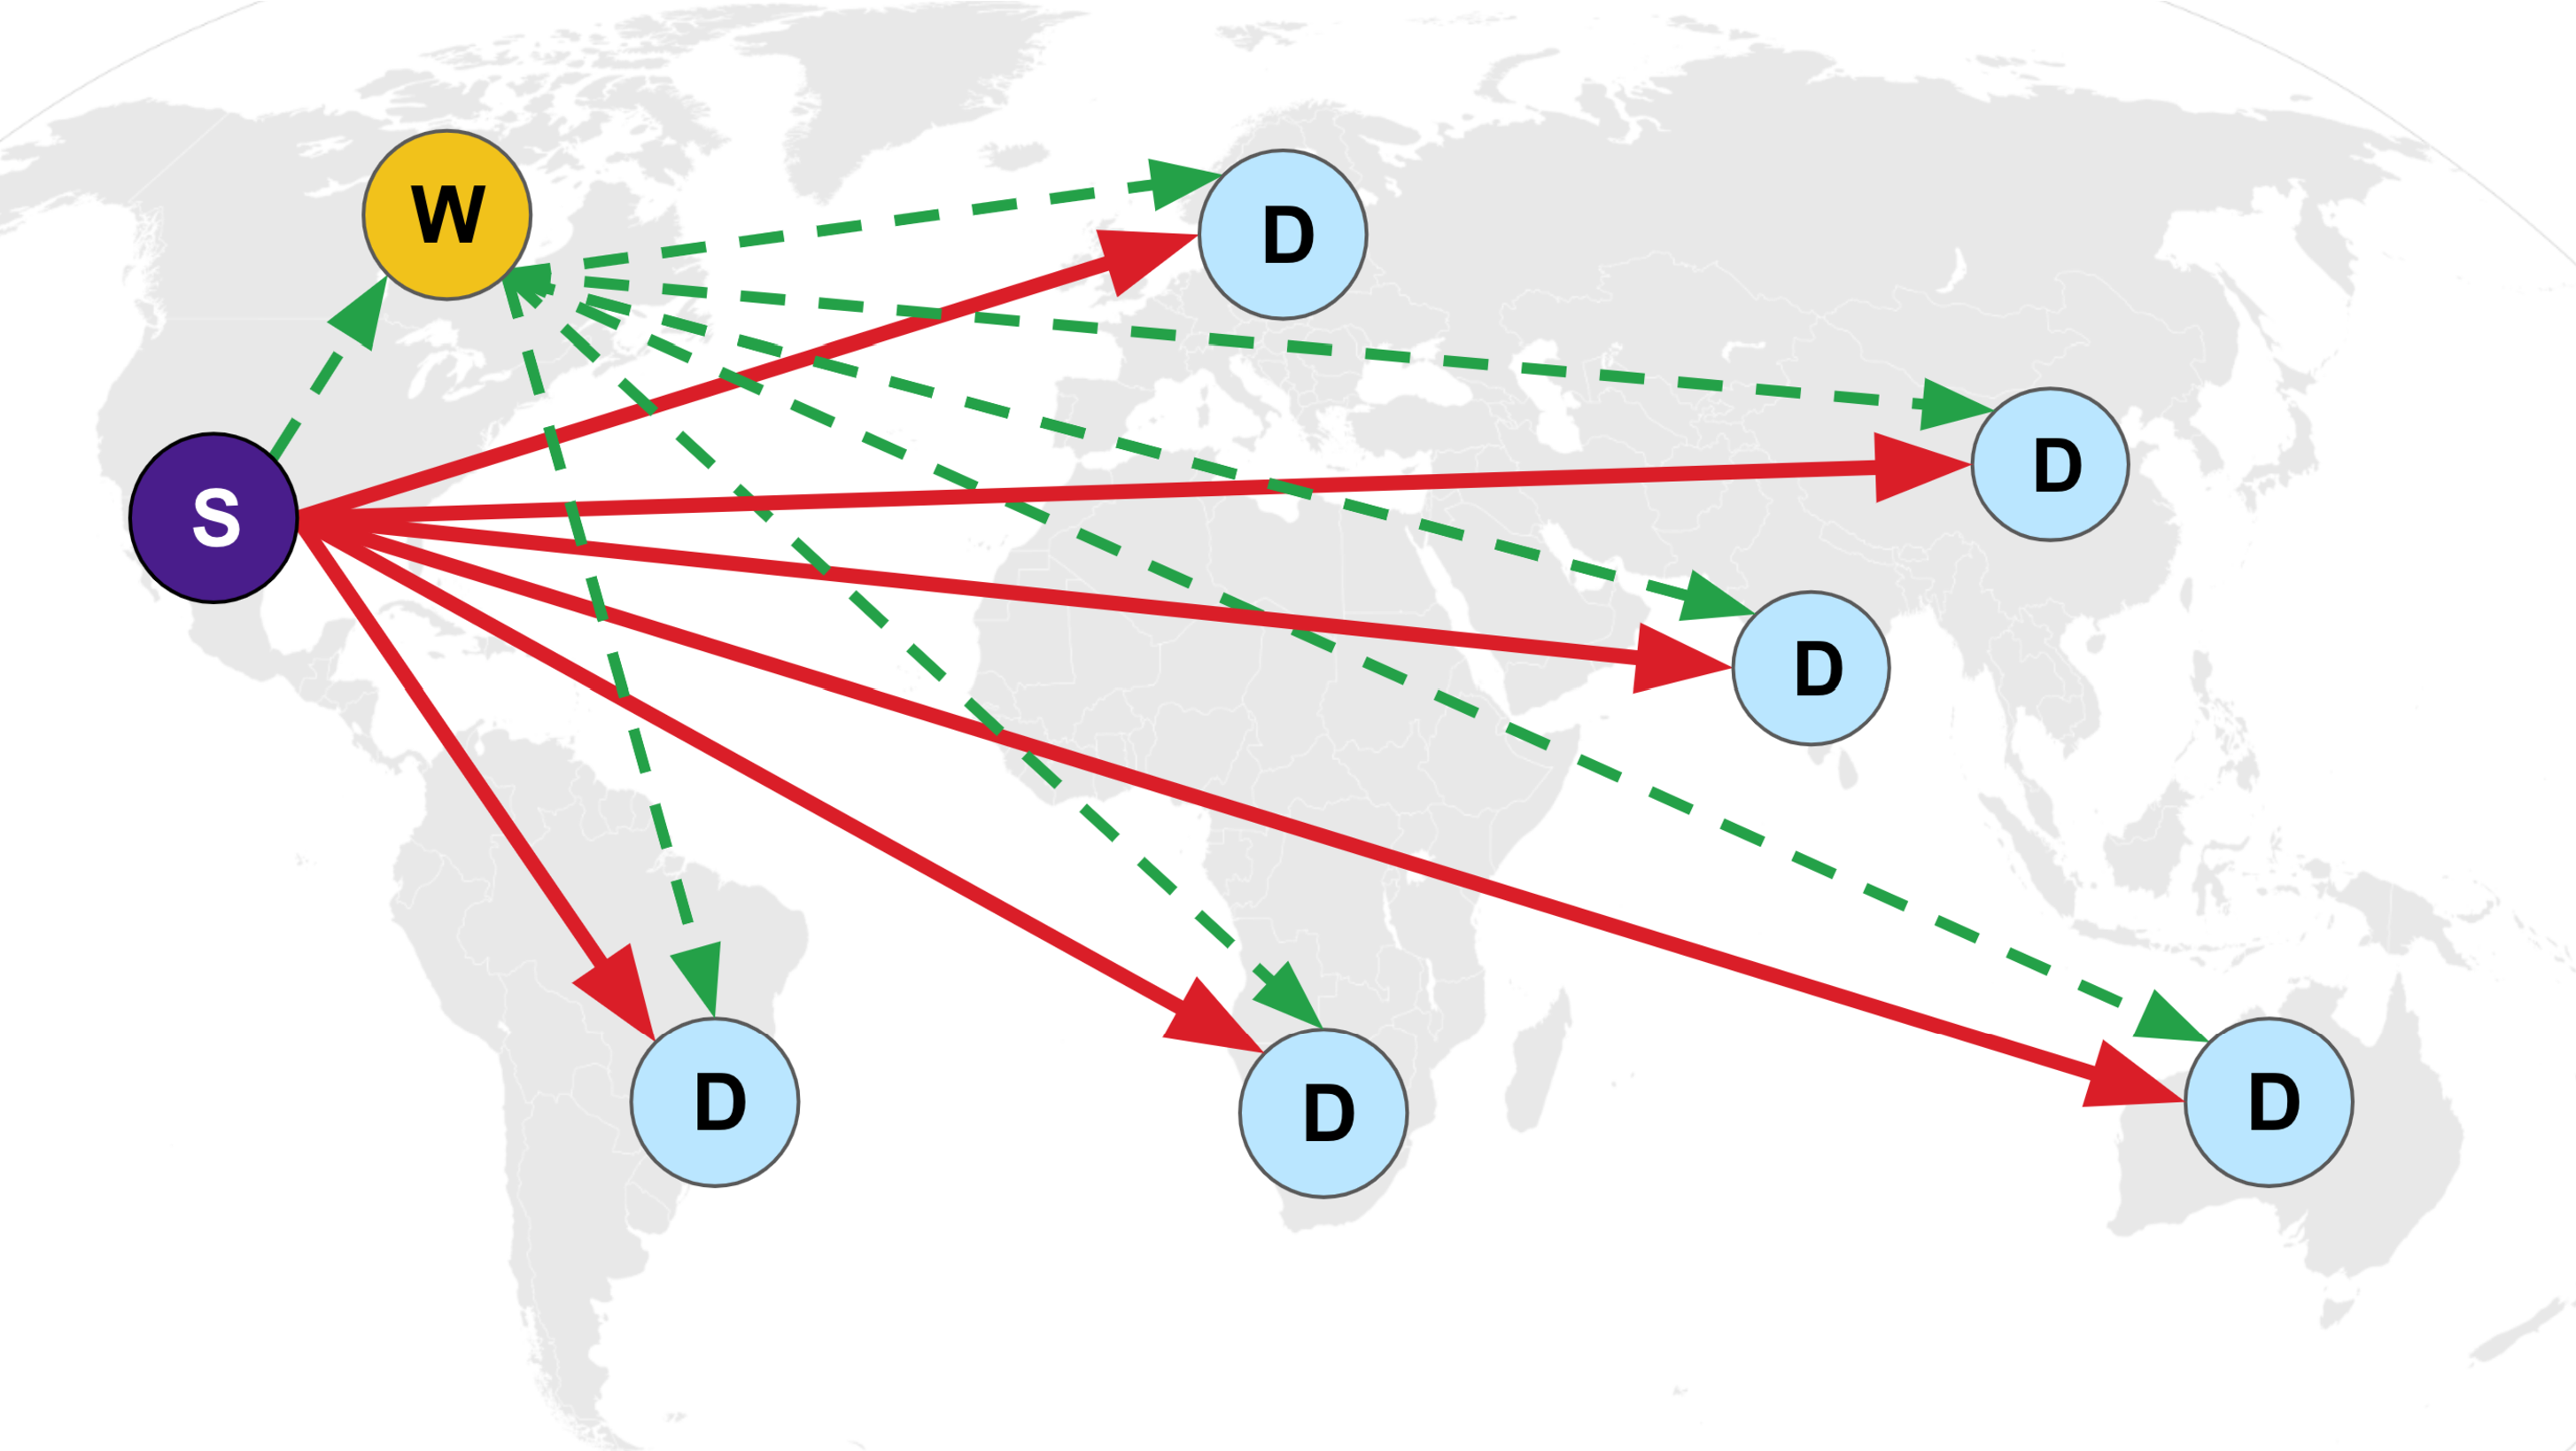
\includegraphics[width=0.8\linewidth]{figures/overview.pdf}
     \caption{Direct replication from a source region (purple) to destination regions (blue) may traverse expensive or slow links, which can be avoided via \textit{waypoint} regions (yellow).}
     % \joey{can we add some more waypoint regions to this plot?}
     \label{fig:overview}
\end{figure}


Egress costs can vary by orders of magnitude depending on the source and destination~\cite{cloudflareegress}, as well as the capacity of cross-region links.
%nd the performance of cross-region links is similarly variable.
%Focusing on throughput alone can, thus, lead to poor results, especially as the number of destinations increases.
As a result, the structure of the multicast replication tree (i.e., what data is replicated along which paths) can dramatically affect the end-to-end throughput and monetary cost of replication.
%
As a concrete example, consider replication from a GCP source region to six AWS regions (Figure \ref{fig:overview}).
%
Direct replication of the data between the source and each destination region (shown in red arrows) would cost $\$720$ per TB. 
%
Instead, replicating to an AWS region with the lowest cross-region egress fees once and multicasting data from that AWS region to other regions (shown in dotted green arrows) would reduce the price to $\$240$ per TB.
%
Further modifying the multicast tree to utilize high-throughput links and offload egress bandwidth from the source node can also improve throughput.

In this work, we solve the problem of \emph{high-throughput, cost-optimized cloud multicast} in which we minimize the cost of data replication while achieving a target replication time (across all destinations) for bulk multicast replication.
%
Cloud multicast incurs costs from network egress fees and compute resources needed to mediate the transfer.
%
In addition, cloud multicast must meet application Service Level Objectives (SLO) for the replication time, such as providing freshness guarantees on replicated data.

We design an optimizer to determine a multicast tree structure given a user-specified source region, destination regions, and target replication time.
By providing varying target replication times, our optimizer can generate a Pareto-curve (shown in Figure \ref{fig:simulated-baselines}) that improves replication cost and throughput compared to prior approaches for cloud multicast \cite{garcia2015cost, ganguly2005fast}. We achieve this by leveraging techniques such as striping, VM parallelism, and overlay networking, while also accounting for the cloud providers' network characteristics, resource constraints, and per-GB network pricing model.

%The key insight in this work is that we can leverage the elasticity of the cloud to design overlay networks of ephemeral virtual machine (VM) waypoints that optimally navigate the path-dependent cloud pricing model to reduce multicast costs and improve throughput significantly. %\joey{I revised this some.}

% Studying the pricing models, resource constraints, and network characteristics of modern cloud providers, we identify opportunities for better multicast tree construction.
% % in cloud replication. 
% We exploit these opportunities using overlay networking techniques to transfer data through ephemeral \textit{waypoint} VMs 
% that are neither the source nor the destination 
% % and may even be in different regions of the world 
% as shown in Figure \ref{fig:overview}.
% We show that the strategic introduction of these waypoints can reduce the overall price of multicast data replication despite using more network bandwidth. % than necessary. 
% %
% Unlike the traditional overlay settings, the cloud offers significantly more flexibility in the number and the location of overlay nodes, as cloud VMs can elastically be instantiated in specified cloud provider regions.


%Our key insight is that transferring data through additional \textit{waypoint} regions, i.e., neither source nor destination regions, can reduce the overall price of multicast replication despite using more network bandwidth than necessary.
%We route data along these price-minimizing replication trees by creating an \textit{overlay network} across cloud regions and providers, which allows us to control the regions and links data traverses through. 

%The cloud context introduces several new challenges: First, cloud pricing for compute and network resources must be considered. Second, cloud resource elasticity enables flexibility in the number of overlay nodes and their location (i.e. on which cloud provider and in which region an overlay node is placed). Third, cloud networks typically have predictable, stable cross-region throughput \cite{jain2022skyplane} and also impose artificial network constraints on VMs, which should be accounted for when designing high-throughput distribution trees.


Designing this optimization is challenging for two main reasons. 
First, the optimizer must account for path-specific pricing models, resource constraints, and varying performance across cloud providers. Existing techniques that formulate the optimization problem in terms of bandwidth allocation cannot be adapted to account for per-GB network pricing without making the problem non-linear (described further in \cref{sec:optimization}). 
%Cloud providers' per-GB network pricing model cannot be easily adapted to prior work optimizing bandwidth-based network costs, which we explain further in \cref{sec:optimization}. 
% to model and optimize multicast price and throughput effectively. 
Second, the optimization search space is combinatorially large, as the optimizer must determine both the set of overlay waypoint regions (regions which are neither the source nor destination) as well as how data will be routed along the overlay network. % (i.e., in the source, destination, and waypoint regions) 
Unlike the traditional overlay settings, the cloud offers significantly more flexibility in the number and the location of overlay nodes, as cloud VMs can dynamically be instantiated in specified cloud provider regions. Furthermore, replicating subsets of data (i.e., stripes) via different paths is critical for achieving high-throughput \cite{castro2003splitstream}.
We introduce several approximations (e.g., pre-selecting the regions and limiting path lengths) to reduce this search space and enable the optimizer to run within seconds.

To run overlay multicast across clouds, we develop \textit{Cloudcast}, a system for bulk data overlay multicast across GCP, AWS, and Azure.
%
Cloudcast has a centralized control plane that supports pluggable algorithms for determining the number and location of overlay nodes and replication trees for multiple segments of data. 
%
We implement our optimizer as well as several baseline algorithms as part of Cloudcast's control plane. 
% We then develop a lightwe % simon: i comment this line out because of the fragment
We run system experiments to multicast data across clouds and show that \sys is able to achieve up to $62.4\%$ cost savings and $2.84\times$ replication speedup depending on the control plane algorithm (Figure \ref{fig:inter-cloud-1}).  

We run an end-to-end system evaluation comparing \sys with  BitTorrent \cite{facebook-bittorrent} and AWS's commercial offering for multi-region bucket replication \cite{awsbucket}, which, like most cloud data replication offerings, only supports replication into or within that cloud.
% 
We find that \sys achieves $7.7\times$ replication speedups and $28.4\%$ cost savings compared to BitTorrent (Figure \ref{fig:p2p_comparison}). Compared to multi-region bucket replication, we find that \sys achieves up to $61.5\%$ cost reduction and $2.3\times$ replication speedup (Figure \ref{fig:aws_comparison}).

%\sys will be open-sourced upon publication. We provide an anonymized tool to explore \sys's optimizer.\footnote{An anonymized website visualizes Cloudcast-optimized overlays for different configurations: \url{https://anon-eurosys-585.github.io} \textcolor{red}{CHANGE ME!!!!!!!!!!!!!!!!}}

\vspace{0.5em}
To summarize, we make the following contributions: 
\begin{compactenum}
    %\item We introduce the problem of \textbf{cost-optimized} cloud multicast and characterize key aspects of cloud pricing models and resource limits that determine optimality.
    % \vincent{missing something about insights into cloud pricing patterns.  More generally, I think something you'll want to push how the structure of clouds and their pricing patterns impacts the optimizer design (to defend against the `it's just an ILP' criticism.}
    
    \item We design an optimizer for minimizing replication cost under replication time constraints. 
    \item We introduce several approximations to reduce the search space for the optimizer, reducing the solver runtime from hours to seconds.
    
    \item We build \sys, an open-source system for cloud overlay multicast with pluggable data transfer policy.
    % \sarah{add footnote}\joey{I think we can skip it for space.}
    %\item We use our optimizer to analyze how cloud pricings affect the cost-minimizing topology solution, especially how future changes on network pricing models (e.g. zero inter-cloud egress) may create new optimization opportunities.
\end{compactenum}


%\ion{Let's be consistent. We are using "dissemination", "distribution", "replication", etc. Let's just use "data replication" everywhere as it has the clearest semantics.} \simon{I fixed it for the intro only.}

% Ion: also consider the priodict solution (less distribution trees) 

% tell Ion when its ready - probably next weekend 
% give eval by sunday 
% evaluation for all stripes versus some of the stripes 
% see difference between the algorithms 
